\subsection{User Flows}
\label{sec:user-flows}

Phần này đặc tả các luồng thao tác chính bằng sơ đồ, so le giữa \textit{định nghĩa hành vi đã chốt} ở ma trận case C1--C9 (bảng~\ref{tab:switch-matrix}) và \textit{ảnh chụp thật từ ứng dụng}. Mỗi luồng được truy vết về user story ở mục~\ref{sec:user-stories} và về kịch bản kiểm thử TC01--TC14 của nhóm.

\textbf{Luồng phiên đầu tiên.} Đây là luồng quan trọng nhất vì quyết định người dùng có ``chạm'' được USP ngay lần đầu mở ứng dụng hay không. Hình~\ref{fig:act-first-run} mô tả luồng này bằng sơ đồ hoạt động theo đúng các con số đã chốt ở mục~\ref{sec:mvp-scope}.



Luồng phiên đầu tiên tuân theo ba nguyên tắc của onboarding: \textbf{giá trị}~--~ba màn đầu chỉ giải thích OneSpace giải quyết được gì (một app thay bốn app chuyên biệt) thay vì khoe tính năng; \textbf{quyền riêng tư}~--~không xin quyền nào lúc mở lần đầu, mọi quyền chỉ hỏi đúng lúc người dùng dùng đến tính năng cần nó; và \textbf{tính liền mạch}~--~chọn chủ đề xong vào thẳng Home với đề xuất theo đúng chủ đề vừa chọn, không bắt đăng nhập trước khi thấy được sản phẩm (chế độ dùng thử luôn có).

\textbf{Xung đột âm thanh (case C1).} Khi người dùng mở một bài nhạc trong lúc video đang phát, ứng dụng hỏi bằng popup hai lựa chọn (tắt tiếng video / dừng video) kèm ô tick ``Không hỏi lại''; lựa chọn áp dụng cho lần đó và lần xung đột sau vẫn hỏi~--~chỉ khi người dùng tích ``Không hỏi lại'' thì lựa chọn đang chọn được ghi nhớ, và đặt lại ``Luôn hỏi'' được trong Cài đặt. Hình~\ref{fig:act-conflict} là sơ đồ hoạt động theo đúng định nghĩa đã chốt; Hình~\ref{fig:app-c1} là popup thật trên ứng dụng.



\begin{figure}[H]
\centering
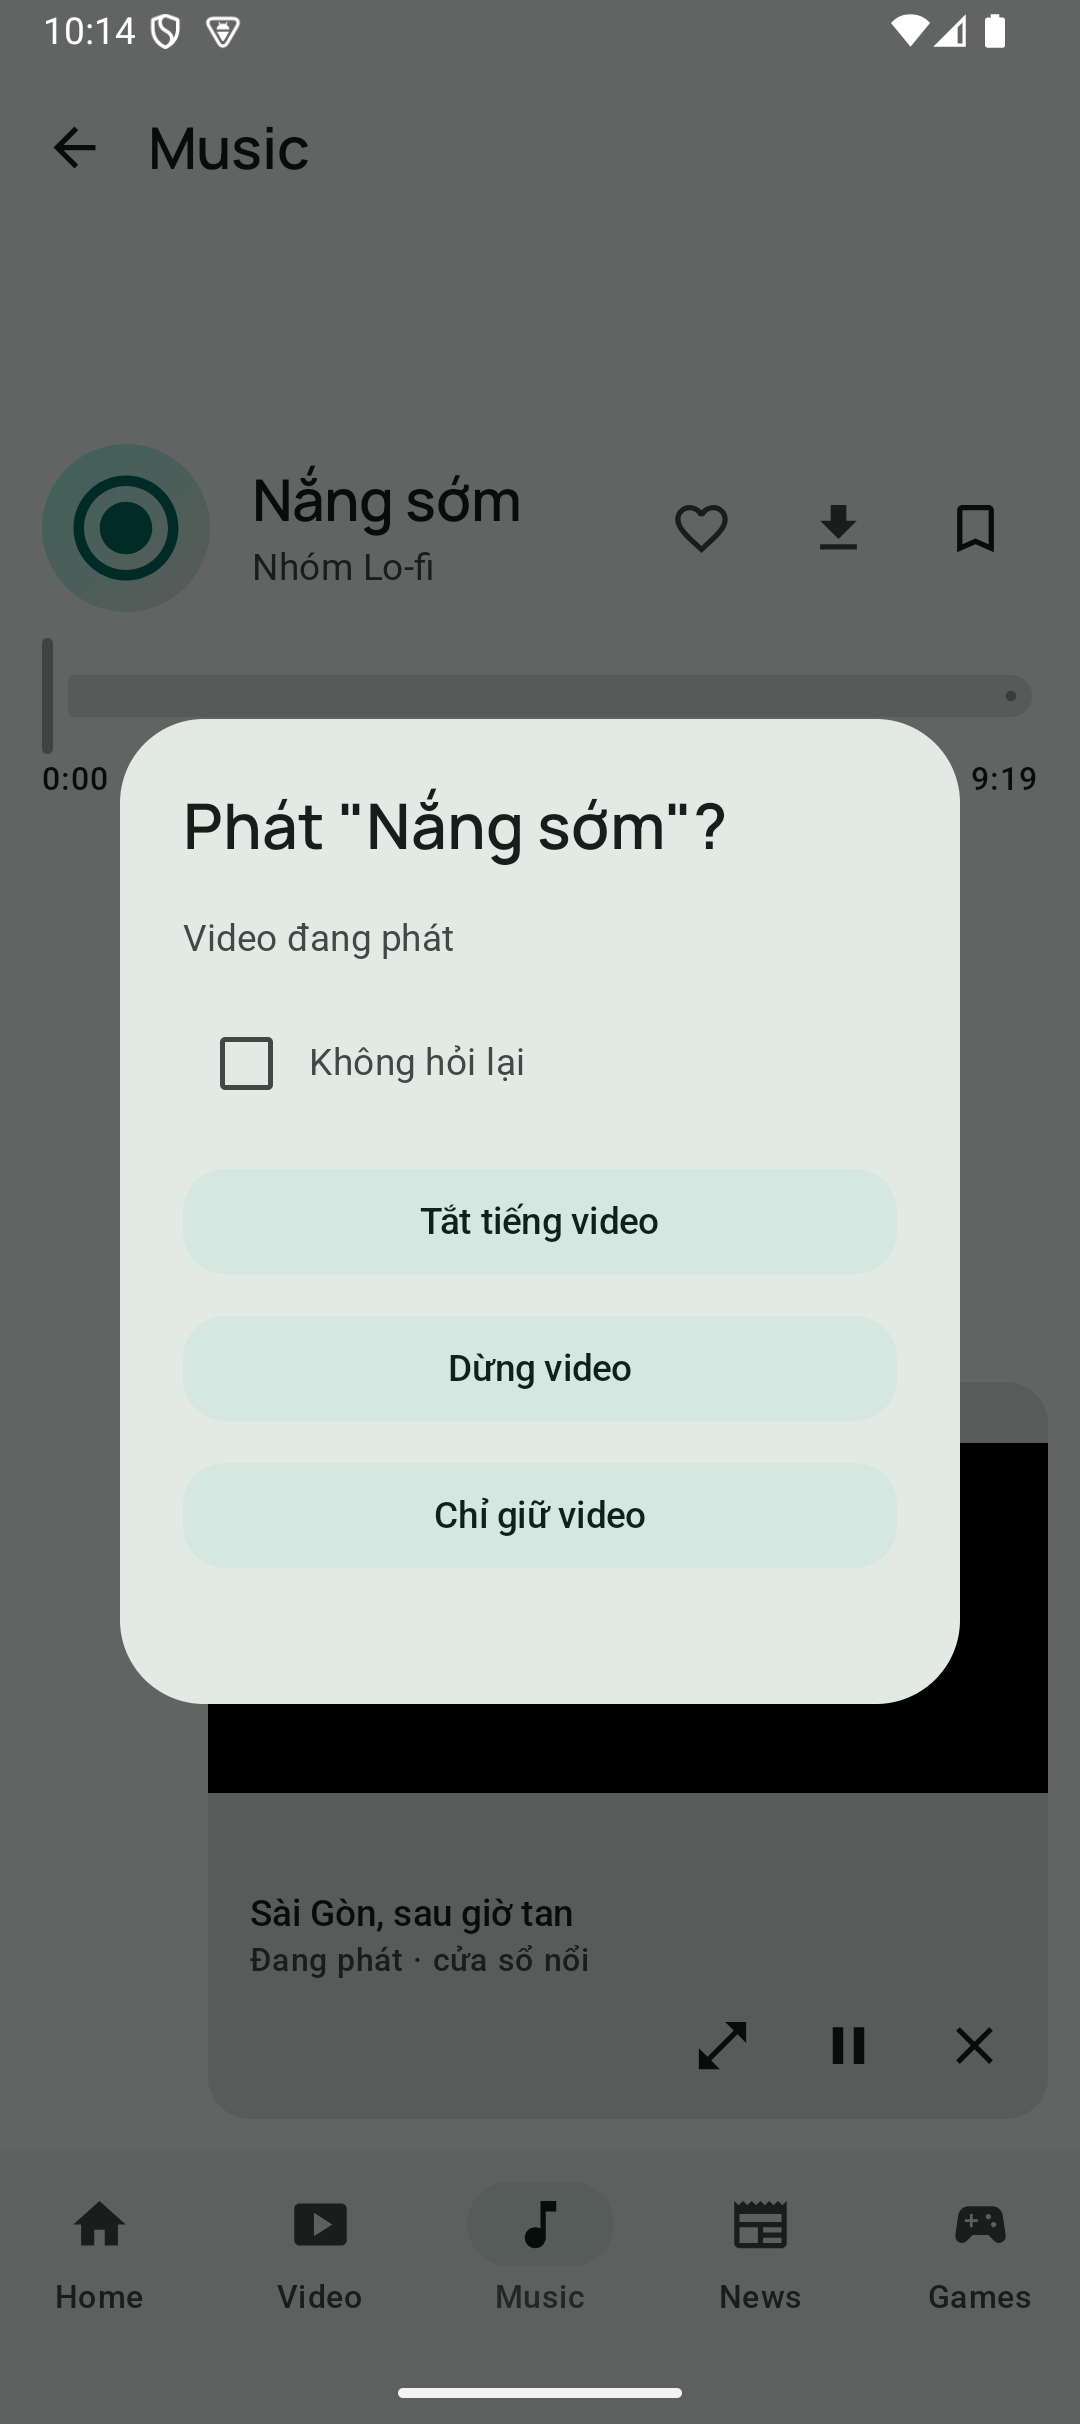
\includegraphics[width=0.28\textwidth]{figures/app/c1-audio-conflict-light.png}
\caption{Popup xung đột âm thanh thật trên ứng dụng: video ``Gần với thiên nhiên thêm chút'' đang phát, người dùng mở bài ``Nơi nào yên tĩnh''}
\label{fig:app-c1}
\end{figure}

Hình~\ref{fig:app-pip} chụp cửa sổ nổi thật đang chạy trên tab News: cửa sổ hiển thị tên video cùng các nút điều khiển, trong đó có Mở rộng, Tạm dừng và Đóng.

\begin{figure}[H]
\centering
\begin{minipage}{0.48\textwidth}
\centering
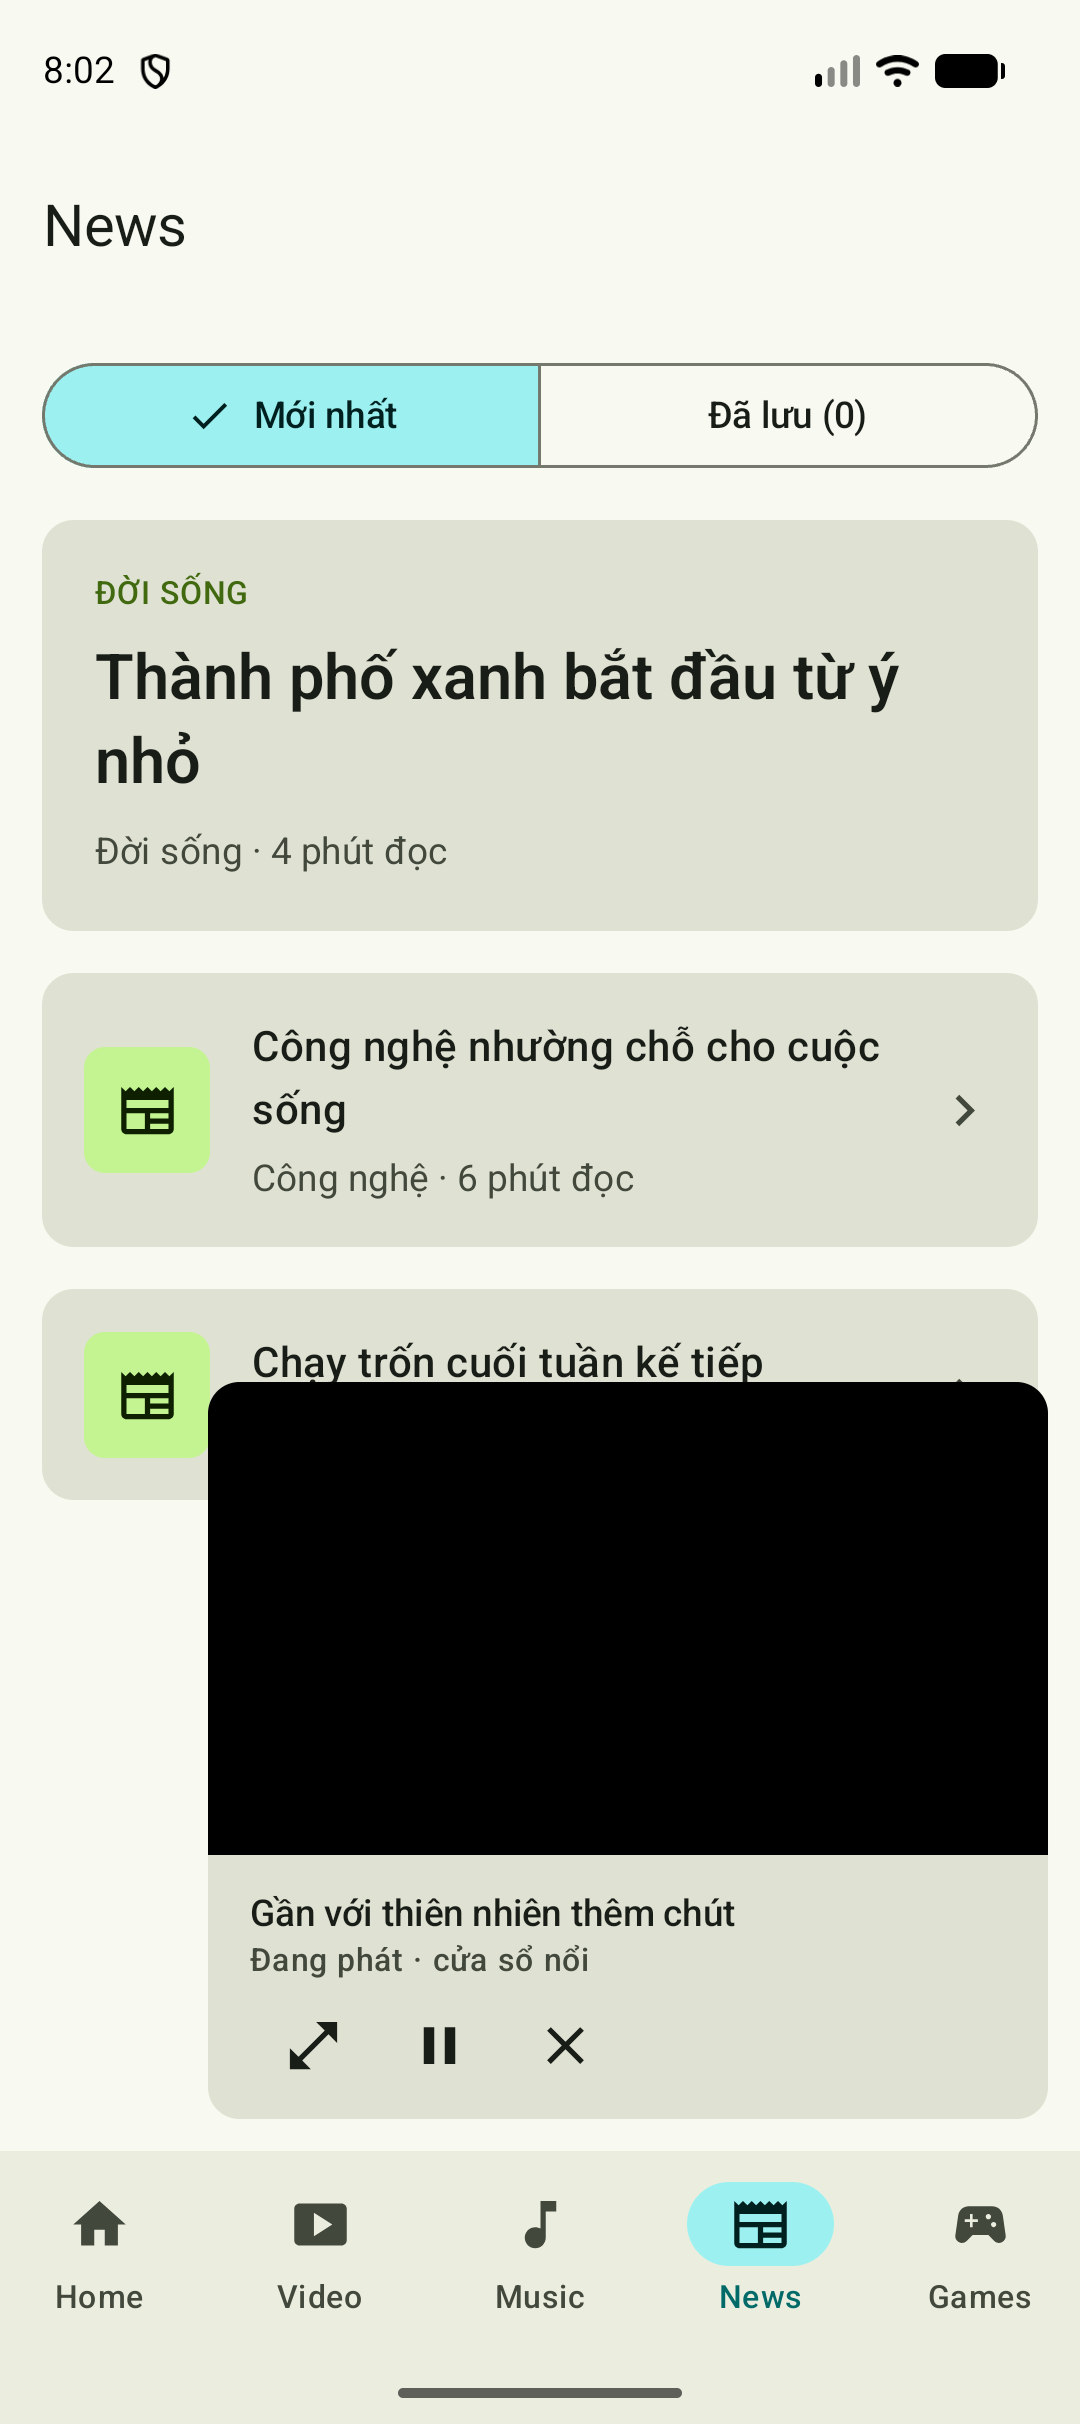
\includegraphics[width=0.55\textwidth]{figures/app/news-pip-light.png}
\caption{Video thu nhỏ thành cửa sổ nổi trên tab News (case C3, F-VID-08)}
\label{fig:app-pip}
\end{minipage}\hfill
\begin{minipage}{0.48\textwidth}
\centering
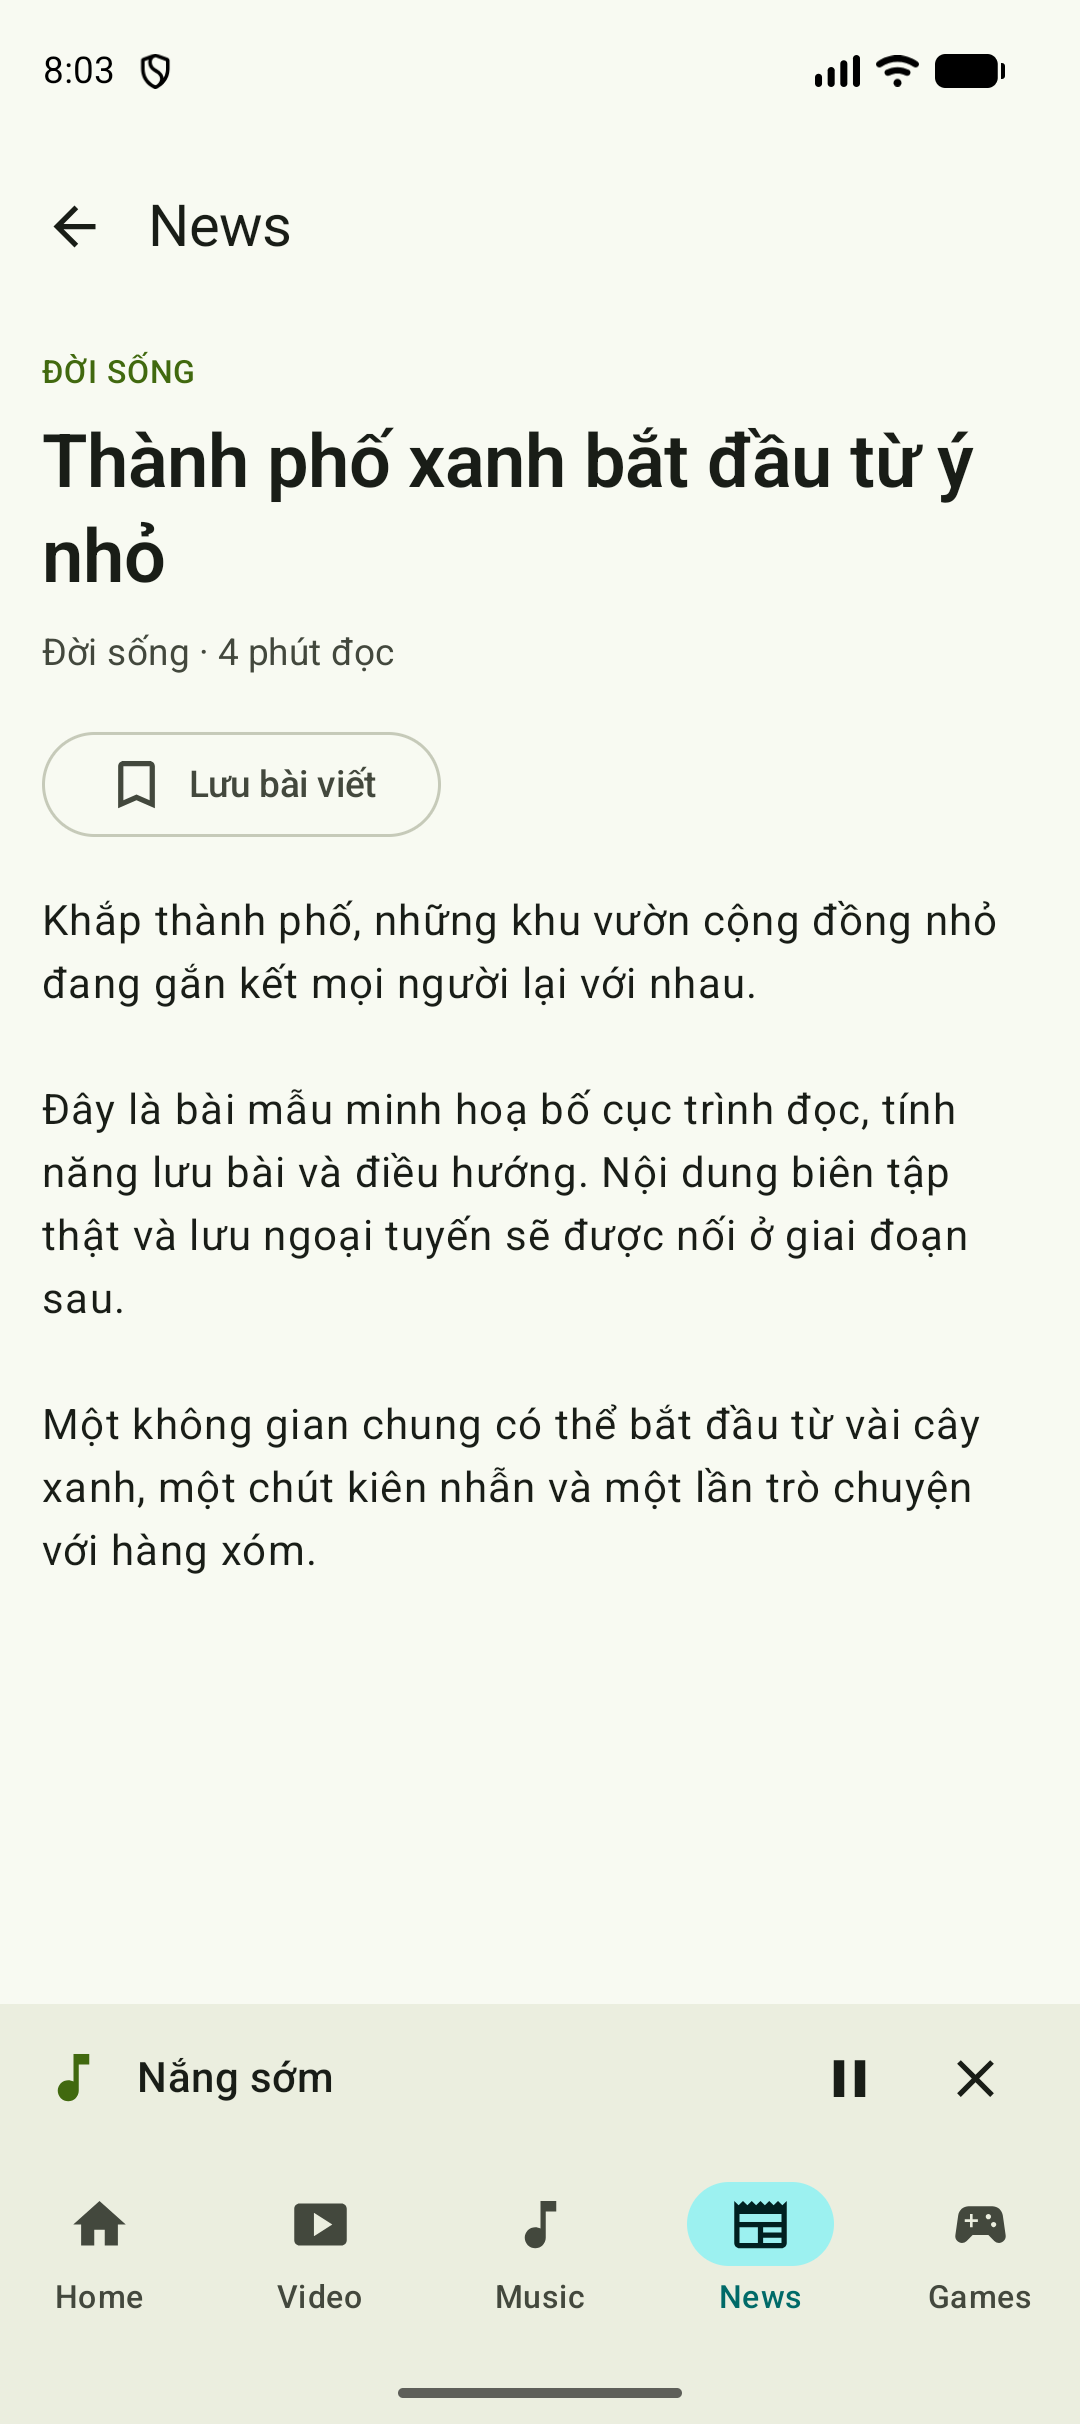
\includegraphics[width=0.55\textwidth]{figures/app/article-music-dock-light.png}
\caption{Dock mini player hiển thị trong trình đọc bài, nhạc vẫn phát khi đọc tin (case C7, F-NEWS-07)}
\label{fig:app-dock-reader}
\end{minipage}
\end{figure}

\textbf{Nghe nhạc khi đọc tin (case C7).} Đi tiếp chiều B$\rightarrow$C của C3, khi nhạc đang phát và người dùng sang tab News, dock mini player vẫn hiện trên feed và cả trong trình đọc bài để nhạc không bao giờ ``biến mất'' ngoài tầm điều khiển (Hình~\ref{fig:app-dock-reader}). Dock luôn hiển thị tên bài và nút tạm dừng; mở rộng dock ra trình phát đầy đủ cũng chỉ là một chạm.

\textbf{Khôi phục trạng thái.} Trong một phiên, SessionCoordinator giữ bài nhạc đang phát, video nổi và vị trí các màn hình khi người dùng chuyển tab. Khi tiến trình bị hệ điều hành hủy rồi mở lại, ứng dụng khôi phục tab cuối, bài nhạc cuối ở trạng thái dừng và danh sách phát; vị trí video trở lại khi người dùng mở lại đúng video đó nhờ checkpoint trong Room (Hình~\ref{fig:seq-restore}). Vị trí đọc tin, ván game dở qua process death và tự phát lại nhạc chưa được lưu, nằm trong danh sách kế hoạch; đây cũng là các dòng được đánh dấu trong bảng kiểm chứng kiến trúc.

Bảng~\ref{tab:flow-trace} tổng hợp việc truy vết từng luồng tới case, user story và bằng chứng tương ứng.

\begin{table}[H]
\centering
\caption{Truy vết luồng -- case -- user story}
\label{tab:flow-trace}
\begin{tabularx}{\textwidth}{>{\raggedright\arraybackslash}p{2.7cm} >{\raggedright\arraybackslash}p{1.4cm} >{\raggedright\arraybackslash}p{4.3cm} >{\raggedright\arraybackslash}X}
\toprule
\textbf{Luồng} & \textbf{Case} & \textbf{User story} & \textbf{Bằng chứng / kiểm thử} \\
\midrule
Phiên đầu tiên & -- & US-COM-02, US-COM-03 & Hình~\ref{fig:act-first-run} \\
Xung đột âm thanh & C1 & US-MUS-03, US-CROSS-02 & Hình~\ref{fig:act-conflict}, \ref{fig:app-c1}; TC02 \\
Video nổi khi rời tab & C3 & US-VID-02, US-CROSS-03 & Hình~\ref{fig:app-pip}; TC01 \\
Nghe nhạc khi đọc tin & C7 & US-NEWS-03, US-CROSS-01 & Hình~\ref{fig:app-dock-reader} \\
Nhạc tiếp tục khi vào game & C9 & US-GAME-01 & Dock vẫn hiện trên tab Games; TC04 \\
Khôi phục phiên (tab, bài cuối, vị trí video) & -- & US-CROSS-07 & Hình~\ref{fig:seq-restore}; TC05, TC10 \\
Mất mạng khi đọc tin / xem video & -- & US-CROSS-07 & mục~\ref{sec:wireframes-prototypes} \\
\bottomrule
\end{tabularx}
\end{table}

\textbf{Các nhánh lỗi và gián đoạn.} Nhánh ngoại lệ được định nghĩa bằng con số cụ thể để kiểm thử kết luận được ngay, thống nhất với bảng~\ref{tab:switch-matrix} và mục~\ref{sec:quality-pillars}: khi mất mạng giữa video, khung hình đứng kèm đếm ngược 5--15 giây tự thử lại; tin đã tải đọc tiếp; game offline chơi tiếp và điểm ghi cục bộ rồi đồng bộ khi có mạng. Khi mạng mất hẳn, feed chuyển sang trạng thái thông báo rõ ràng kèm nút ``Thử lại'' thay vì để màn hình trống trơn — trạng thái này được mô tả trong mục~\ref{sec:wireframes-prototypes}. Rút tai nghe: nhạc dừng ngay, không tự phát ra loa ngoài (TC12); cuộc gọi đến: mọi luồng nhường trong tối đa 0,5 giây và quay lại đúng chỗ sau cuộc gọi (TC11). Riêng nhánh ``nội dung chỉ dành cho tài khoản Premium'' không xuất hiện trong phiên bản đầu vì MVP phát hành miễn phí, không quảng cáo và không gói trả phí (quyết định ở mục~\ref{sec:mvp-scope}).
